% Uživatelským požadavkem je dynamické zařízení sloužící například jako identifikátor hráče, nebo jako herní nástroj.
% Mělo by ale být schopno zastat i~roli statického zařízení, pro případy her na delších výletech, kde by bylo nepraktické nosit s~sebou velké zařízení.
% Vyžaduje tedy dostatečnou mobilitu, aby uživateli nepřekáželo v~pohybu.
% Zároveň by zařízení mělo být co nejlevnější pro možnost nasazení ve velkém počtu.
% Z~toho plynou požadavky na výslednou konstrukci a velikost zařízení.

% Zařízení by mělo být schopno komunikovat s~ostatními zařízeními, ať už statickými nebo dynamickými.
% Potřebuje také světelný výstup pro zobrazování herních stavů a~jednoduchý vstup pro ovládání.

% % realizace

Pro přehled by zařízení mělo mít jméno a protože muže často sloužit podobne jako semafor začal sem mu říkat semisemaf.

Vstup bude realizován pomocí dvou tlačítek a šestiosého IMU, pro možnost púoužívání gest.

Světelný výstup bude realizován pomocí dvanácti RGB LED uspořádaných do kruhu.
Číslo dvanáct bylo zvoleno aby korespondovalo s hodinami, např. pro hry kde probíhá nějaký odpočet.

Abych nebylo nutné starat se o baterii, bylo napájení zajištěno pomocí USB-A konektoru a~malé powerbanky která se tak dá třeba i snadno vymněnit za nabitou.

\section{Výběr součástek}
Protože zařízení bude vyráběno u firmi JLCPCB je výhodné využívat součástky které mají ve své nabídce.
Dají se sice zařídit aby firma osadila i součástky od externího dodavatele ale je to o něco složitější a je tak jednoduší se tomu vyhnout.

Aby nebylo nutné pro práci se semaforem a AHS je výhodné použít stejný kontroler nebo alespoň kontroler ze stejné rodiny.
Proto byl zvolen kontroler ESP32-C3-MINI-1 který je ve srovnání s ESP32-S3 vírazne levnejší a aplikaci plně dostačuje. 
ESP32-S3 má stejně jako ESP32-S3 USB periferii, která se dá využít na programování kontroleru.
I~tady je ale problém, že se tato metoda dá softwarově narušit a~semisemaf je proto vybaveno stejným programovacím konektorem jako ESP32-S3 na AHS.

Protože mám dobré zkušenosti s inteligentními ledkami WS2812 zvolil jsem na ledk kruh jejich typickou pětimilimetrovou variantu.

Protože IMU by na semaforu nemělo sloužit pro žádná přesná měření ale jen např. pro detekci detekci plácnutí nekoliv jeho síli nebo rychlosti, nezáleží tolik na jeho přesnosti.
Při jeho výběru šlo proto primárně o cenu a zvoleno bylo LIS2DH12TR \cite{LIS2DH12TR}, které komunikuje po SPI.

Kontroler ESP32-C3 i LIS2DH12TR má rozsah napájecího napětí do \(3.6 [V]\) \cite{ESP32C3}\cite{LIS2DH12TR}.
Není proto možné je napájet přímo z napětí na USB na kterém je napětí \(5 [V]\) a bude tedy potřeba něnč.
ESP32-C3 požaduje zdroj se schopností dodat \(0.5 [A]\) \cite{ESP32C3} a jeho typické spotřeba ze skušenost nepřesáhne \(200 [mA]\), LIS2DH12TR pak vyžaduje zanedbatelných \(185 [uA]\) (v závislosti na vzorkovací frekvenci i mnohem méně \cite{LIS2DH12TR} strana 17 tabulka 12).
Považuji proto za vhodné pro jeho napájení použít LDO.
Z nabídky JLCPCB byl proto zvolen LD39200 \cite{LD39200} pro jeho elektrycké parametry a~malé pouzdro.

\section{Návrh schematu a DPS}

Doplnil jsem blokovací kondenzátory dle doporučení výrobců, pull-up rezistory na~straping pin kontroleru, spětnovazební dělič k LDO, k~tlačítkům sem připojil debounce kondenzátor a~dostal schéma jsem schéma \ref{semisemafor-sch-v1}.

Ze schematu jsem nakreslil DPS \ref{semisemafor-pcb-v1}

\begin{figure}[!h]
  \begin{center}
    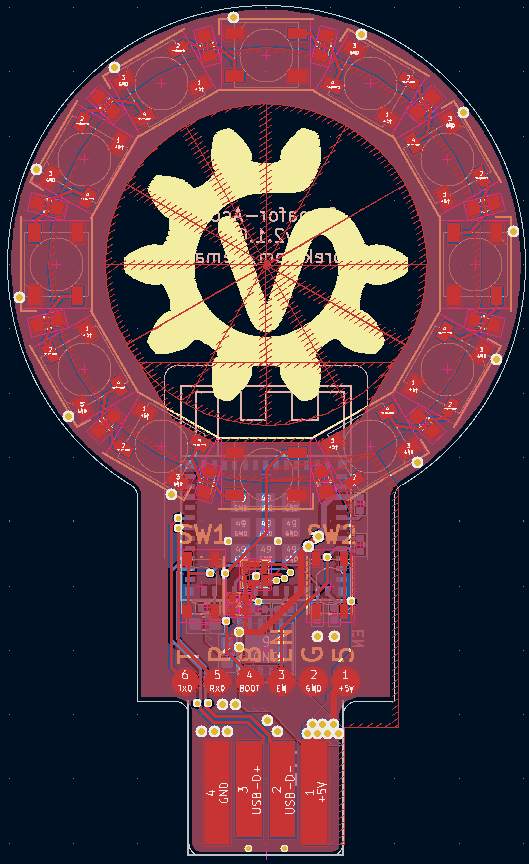
\includegraphics[width=0.7\textwidth]{text/PraktickaCast/img/SemiSemafor-PCB-V1.png}
  \end{center}
  \label{semisemafor-pcb-v1}
    \caption{Puvodní DPS Semisemaforu}
\end{figure}

\begin{figure}[!h]
  \vspace{-20mm}
  \hspace{-10mm}
  \hspace{-10mm}
  \begin{minipage}{1.0\textwidth}
    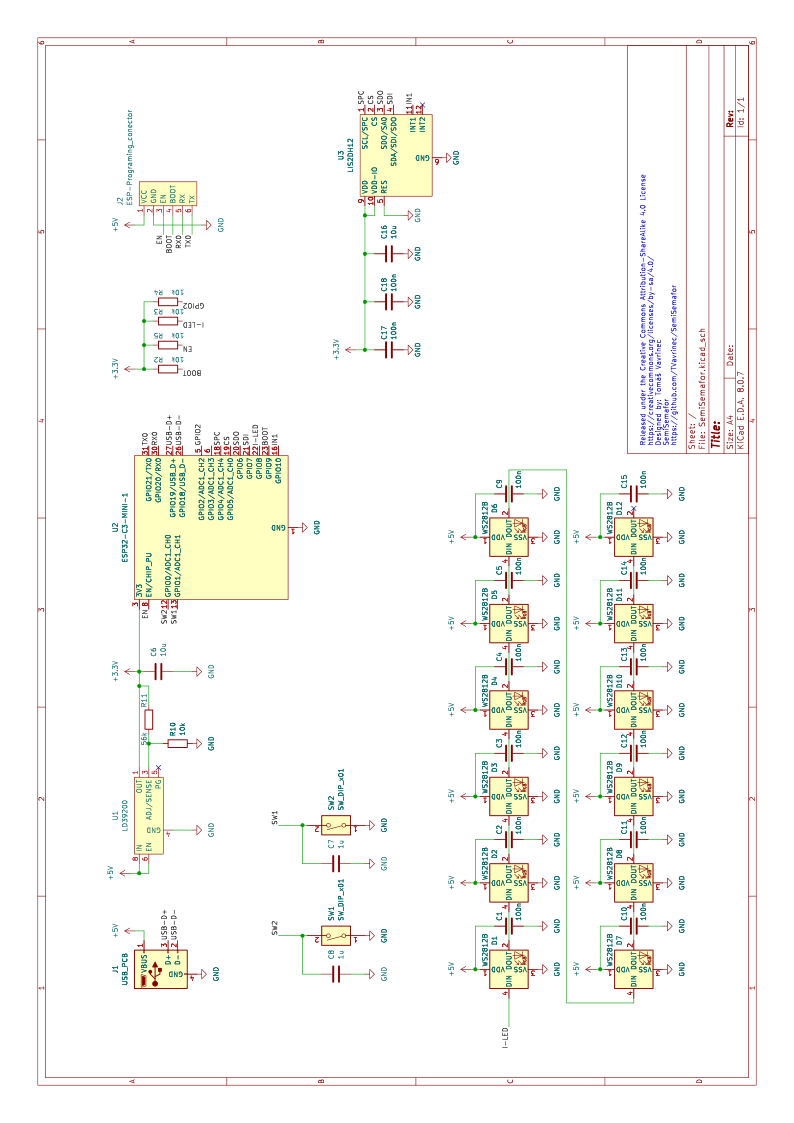
\includegraphics[width=1.2\textwidth]{text/PraktickaCast/img/SemiSemafor-SCH-V1.png}
    \label{semisemafor-sch-v1}
    \caption{Puvodní schéma Semisemaforu}
  \end{minipage}
\end{figure}

\clearpage
\newpage
\newpage


\section{Prototypy}

Při testování první verze, byl problém s neovladatelnými ledkami.
Při pokusu o nastavení barvy se jen náhodně rozsvěcovali a zhasínali.
Když jsem připojil osciloskop na jejich řídící signál, obdržel jsem signál \ref{semisemafor-zvonek} % TODO: změřit znovu a dodat hesží graf

\begin{figure}[!h]
  \begin{center}
    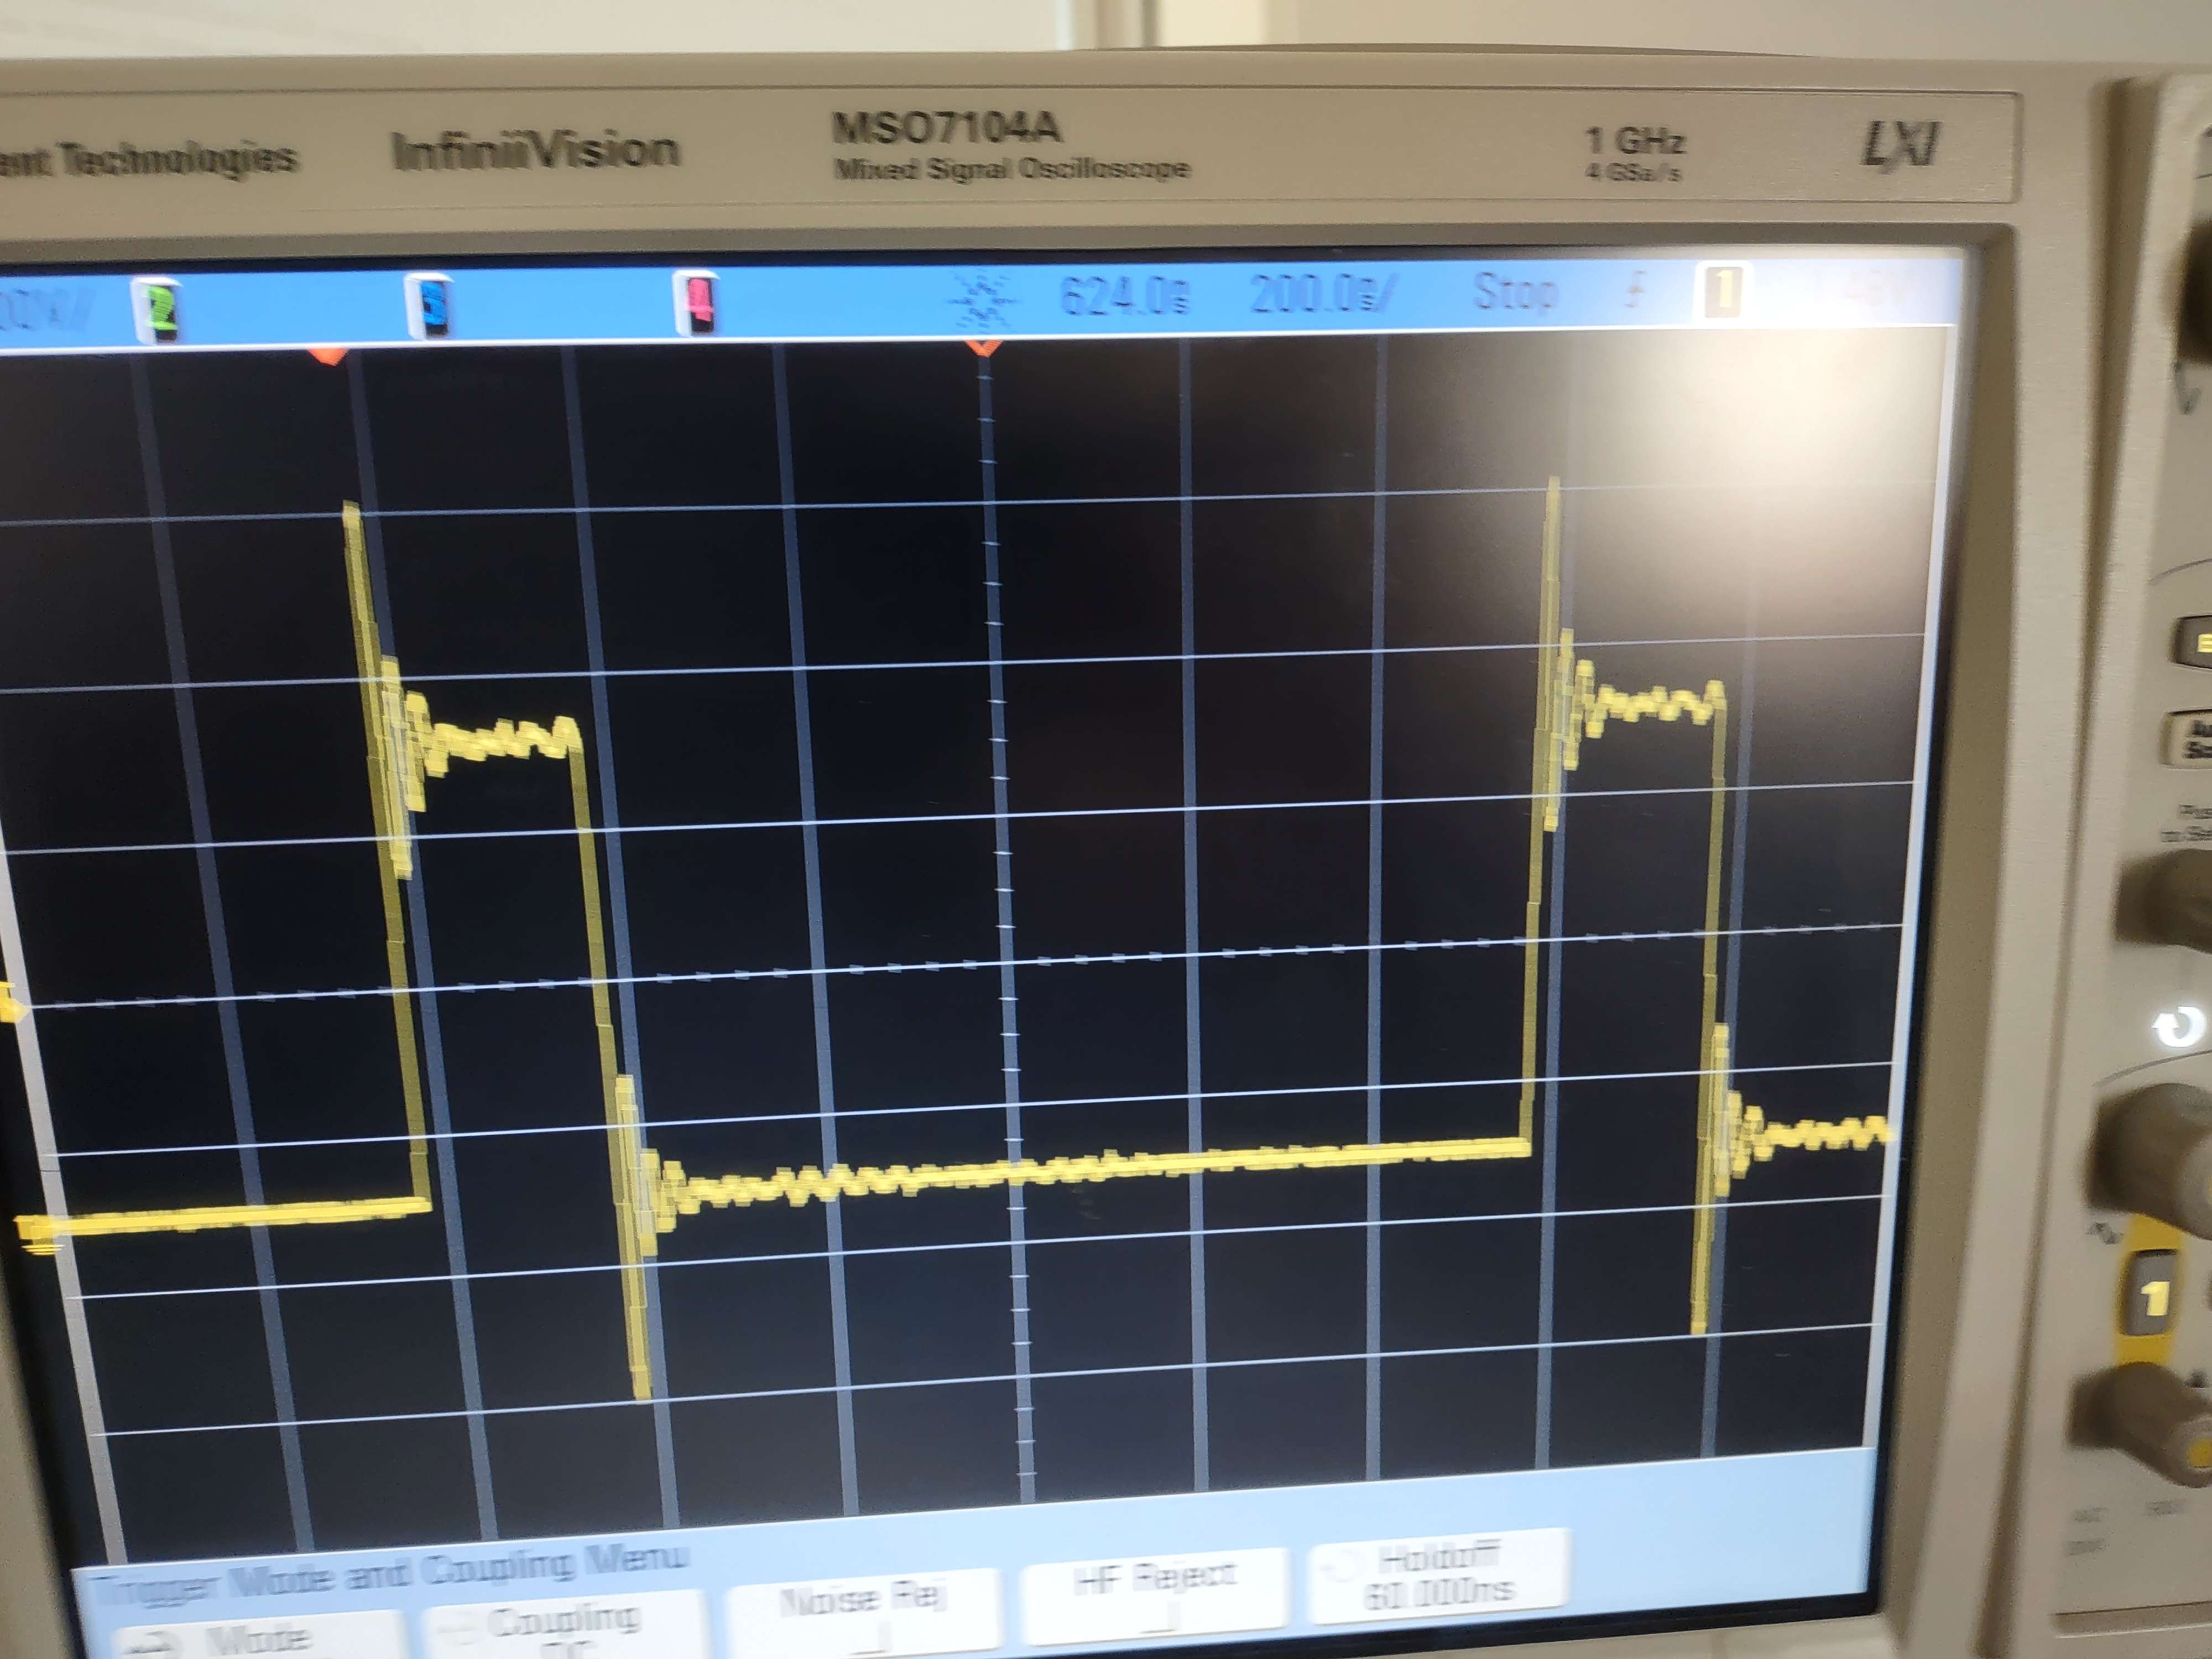
\includegraphics[width=\textwidth]{text/PraktickaCast/img/trampolina.jpg}
  \end{center}
  \label{semisemafor-zvonek}
  \caption{Zarušená komunikace s ledkami}
\end{figure}

Tento problém jsem vyřešil doplněním feritu do cesty řídícího signálu, abych utlumil vyšší harmonické složky.

Kvuli servisním zákrokum a vzhledu krytu jsem navíc přidal i další dvě kontaktní plošky pod USB konektor pro možnost přehrání firmwaru bez nutnosti vijmutí desky.
Vísledné schém \ref{semisemafor-sch-v2}

\begin{figure}[!h]
  \vspace{-20mm}
  \hspace{-10mm}
  \hspace{-10mm}
  \begin{minipage}{1.0\textwidth}
    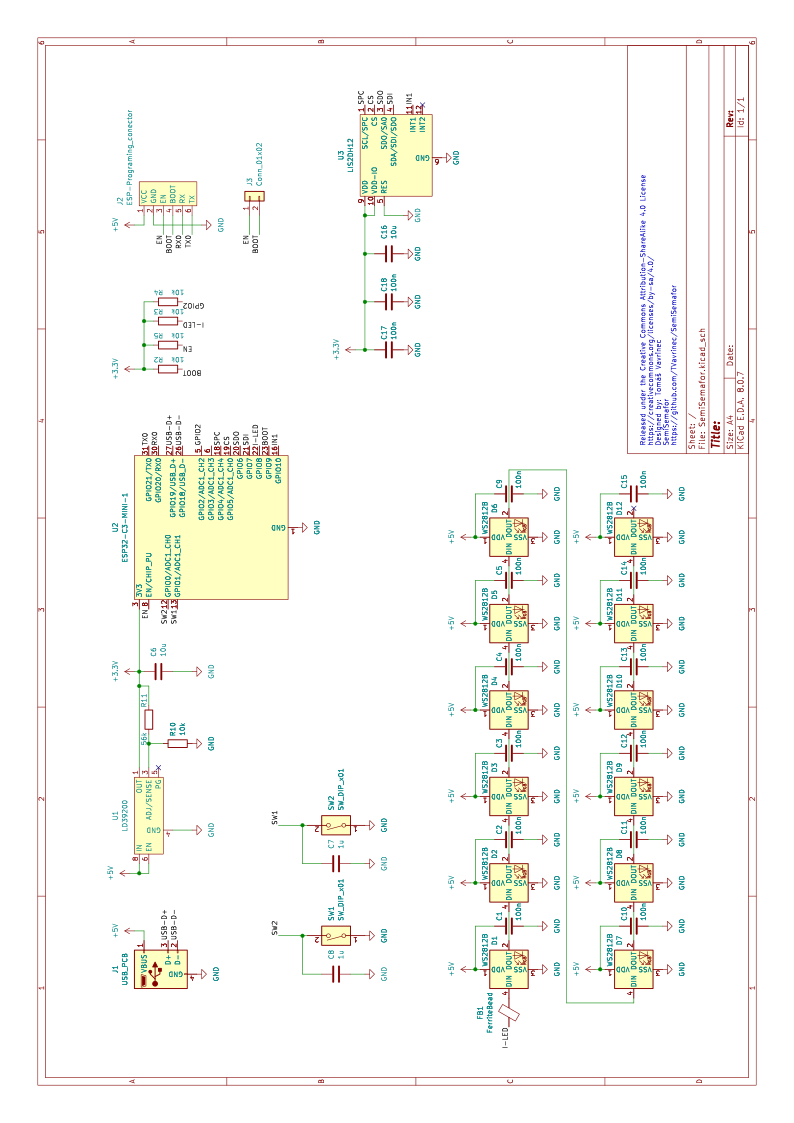
\includegraphics[width=1.2\textwidth]{text/PraktickaCast/img/SemiSemafor-SCH-V2.png}
    \label{semisemafor-sch-v2}
    \caption{Výsledné schéma Semisemaforu}
  \end{minipage}
\end{figure}

\clearpage
\newpage
\newpage

\clearpage
\newpage
\newpage

\section{Mechanické stavba}
Jedním z podstatných požadavků byla jistá uroveň kdytí proti vodě, aby se zařízení dalo používat i za deště.
To nutně neznamená uplnou vodotěsnost, dá se totiž předpokládat že zařízení bude používání v poloze kdy je powerbanka dole a Semisemafor nahoře.
Stečí tedy zajistit těsnost proti stékající vodě jen v jednom směru.

Navíc se během testování objevil ještě požadavek na zpětnou vazbu tlačítka v podobě jeho kliknutí. 
Uživatel totiž musí vědět že tlačítko skutečně stiskl na což je mechanická odva samotného tlačítka ideální.

Po několika iteracích jsem obdržel výsledný vzhled (viz obrázek \ref{semisemafor-box-render})
\begin{figure}[!h]
  \begin{center}
    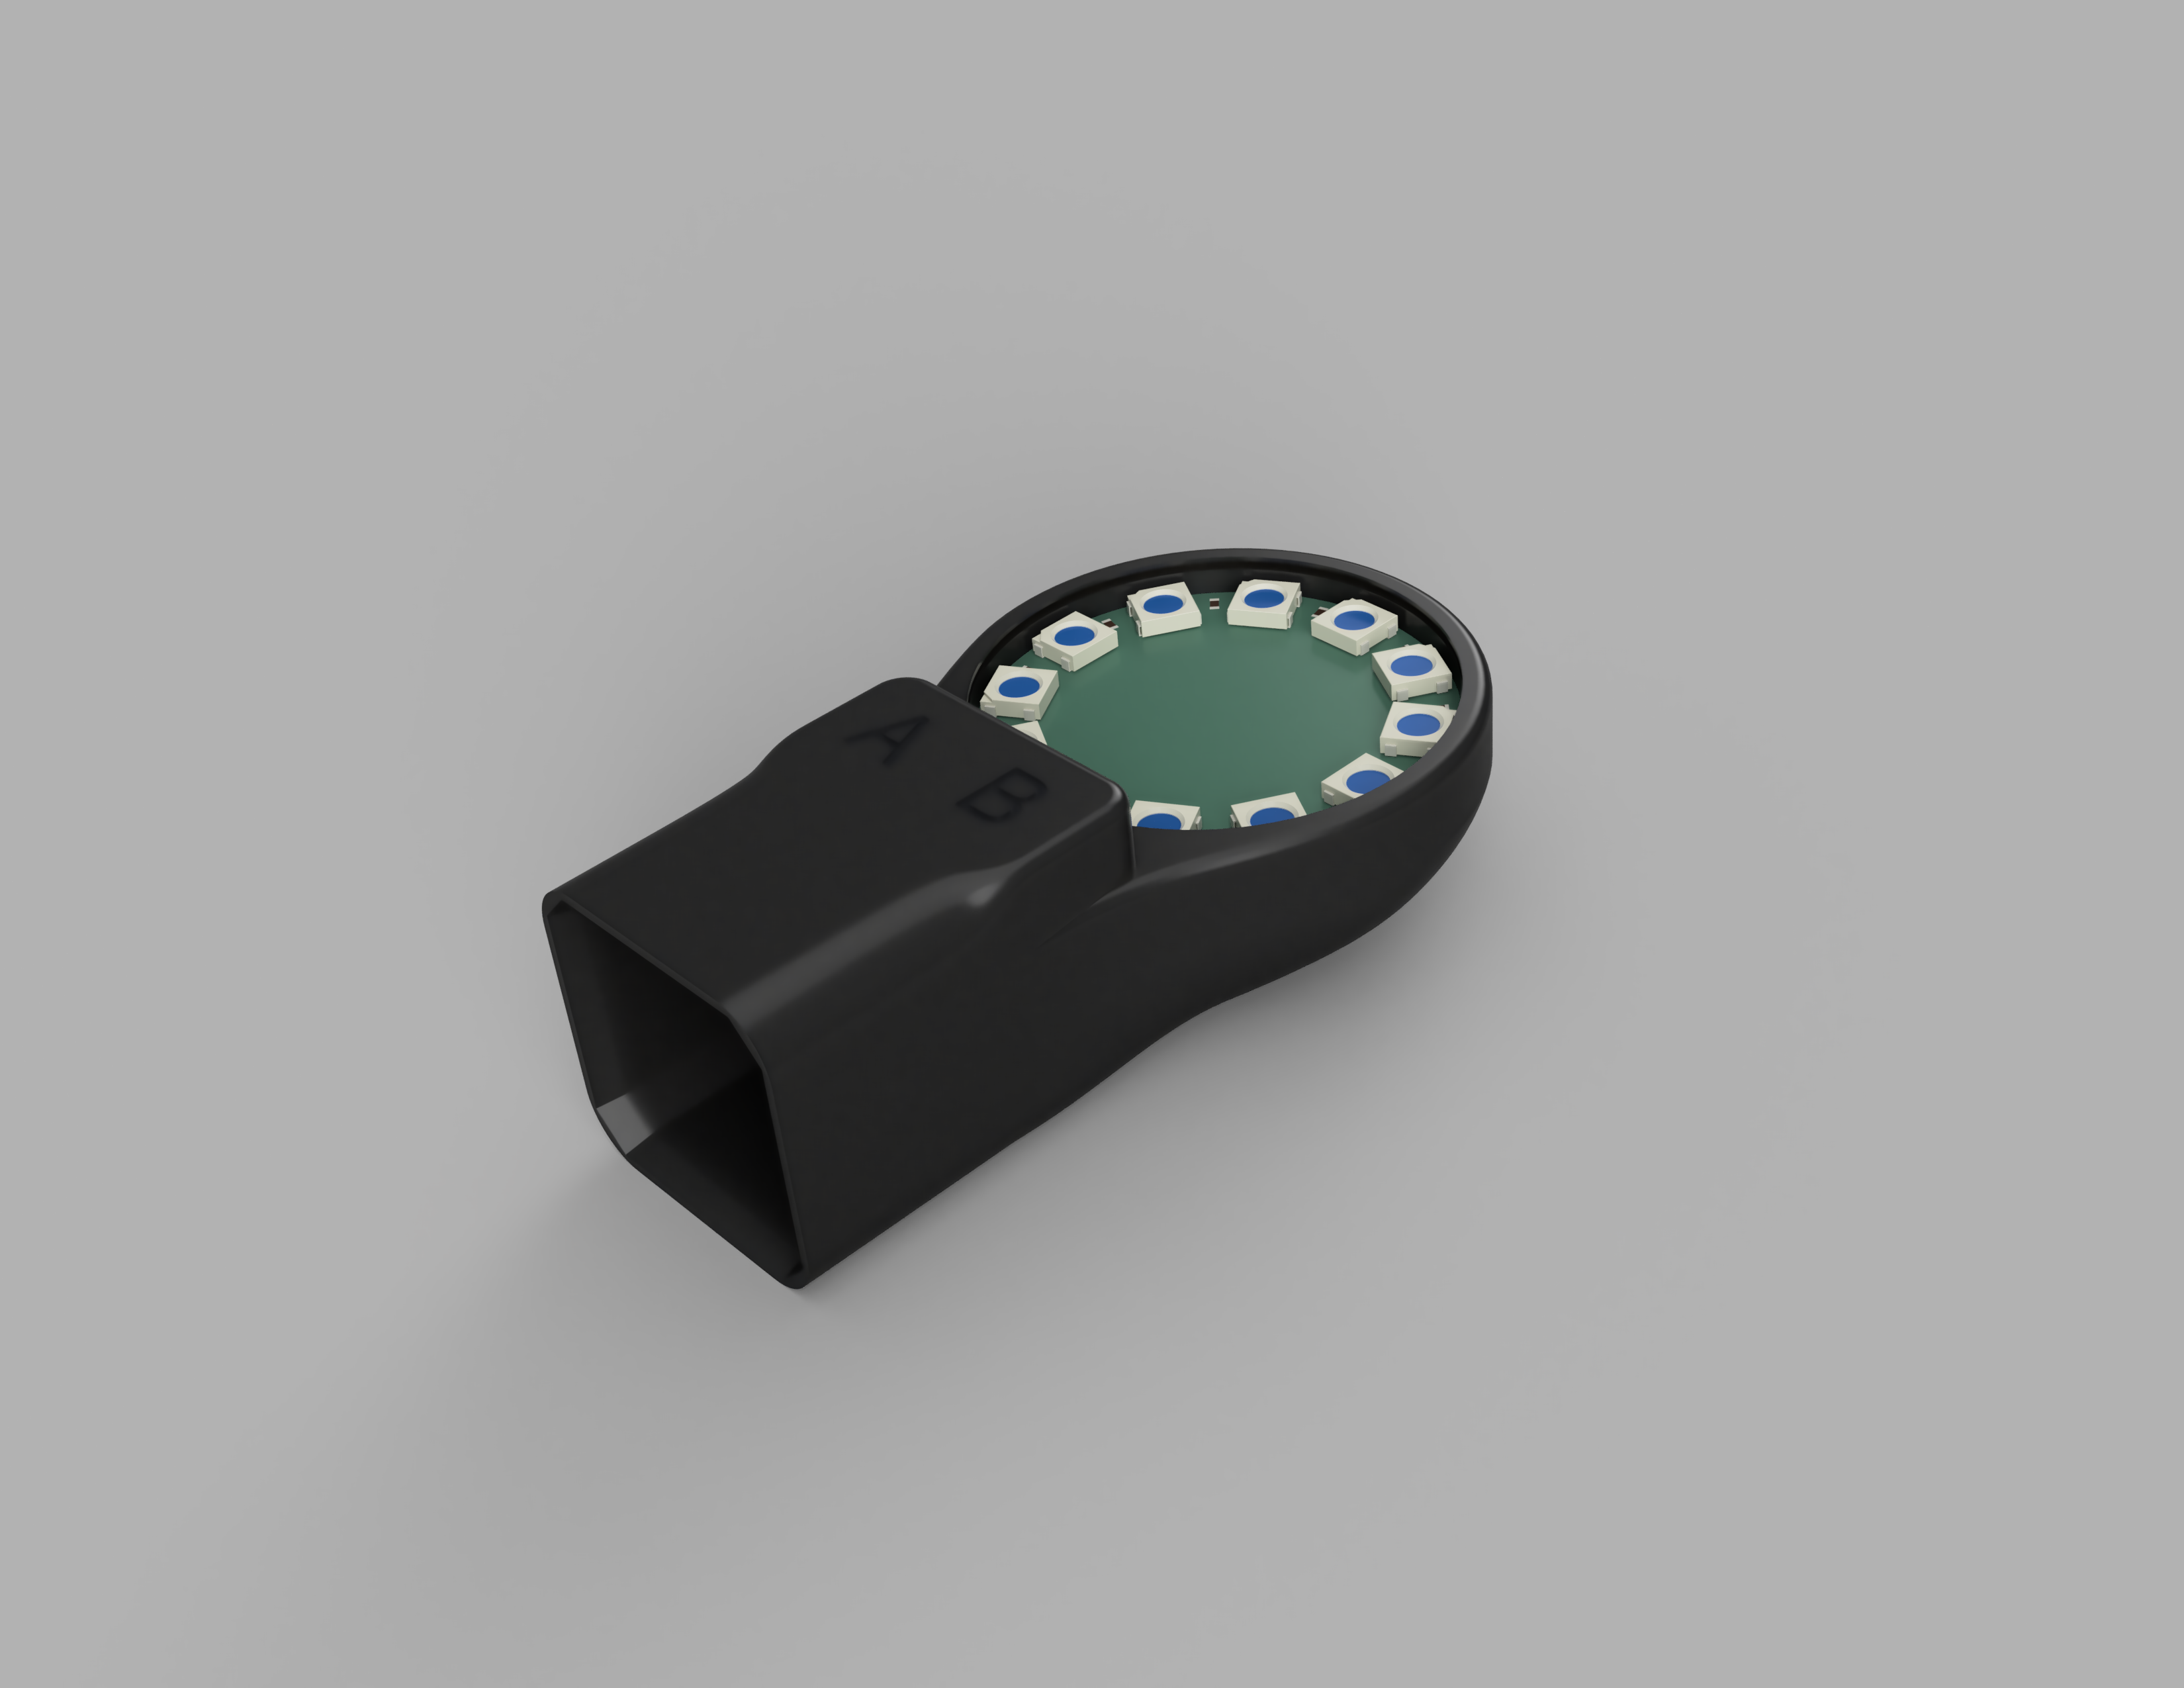
\includegraphics[width=0.7\textwidth]{text/PraktickaCast/img/SemiSemafor-BOX-render.png}
  \end{center}
  \label{semisemafor-box-render}
  \caption{Vzhled Semisemaforu}
\end{figure}

Jako technologii výrobi jsem zvolil obyčejný FDM 3D tisk.
Puvodně jsem chtěl použít materiál SLS pro jeho UV odolnost ale ukázalo se že jsem nebyl schopen navrhnout mechanický vzhled tak aby byl výsledek dostatečně voděodolný a zároveň měli tlačítka uspokojivou zpětnou vazbu.
SLS bylo příliž tuhé a cvaknutí mikrospínače příliž utlumilo aby jej uživatel zaznamenal.
Stejné výsledky jsem měl z PETG, PLA, ABS a nekolika dalšími materiáli, jediný materiál u kterého jsem dosáhl uspokojivích výsledku byl PP (polypropylene).

Problém tisku polypropylenu je jeho tepelné roztažnost takže pokud se tiskne za běžných teplot tak má tendenci se při tisku kroutit což značně zesložiťuje jeho tisk.
Jednou možností by bylo celí tisk provádět při teplotě přez \(120°C\) kde začíná probíhat rekristalizace a polypropylen se začíná výrazně smršťovat.
Tato možnost ale nese nutnost použití speciální tiskárny který umožnuje tiskový prostor vytopit na tak vysokou teplotu a proto byla zvolena méně spolehlivá ale jednodužší metoda.
Použitá metoda je založena na vícemateriálovém tisku, přičemžprimární je užitečný tisknutý objekt z polypropylenu a druhý dobře tisknutelný materiál tvoří podpěry a přítlak.
Aby tak bylo možné vytisknout i tvar který nemá vhodné místa pro umístění přítlaku musí být opatřen technologickýmy výstupky které se po ticku mohou odříznout.

Tiskový model byl tedy doplněn o další objekt zajišťující přítlak a~zároveň i~podpěry.
Výsledek je vidět na obrazku \ref{semisemafor-box-pritlak}

\begin{figure}[!h]
  \centering
  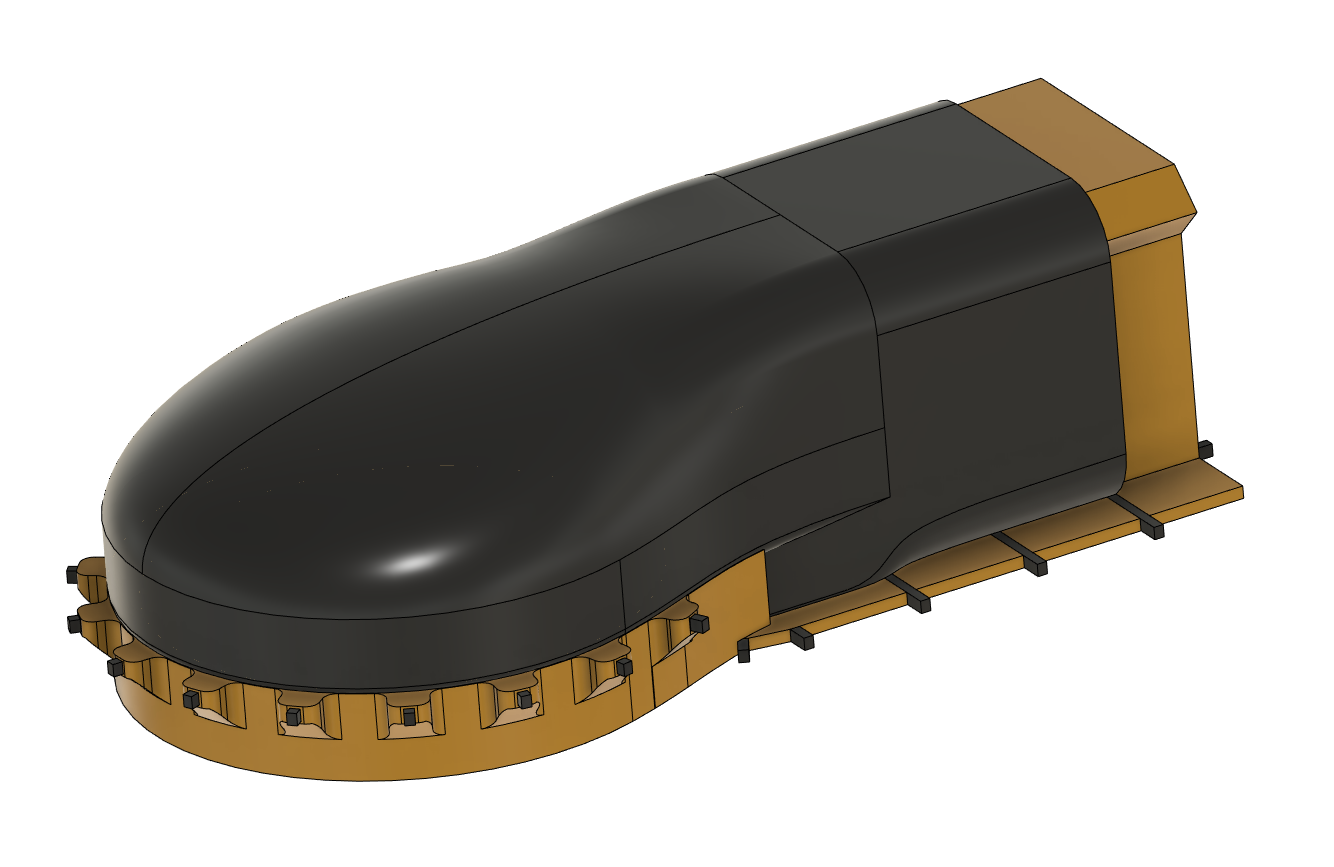
\includegraphics[width=0.7\textwidth]{text/PraktickaCast/img/SemiSemafor-BOX-pritlak.png}
  \label{semisemafor-box-pritlak}
  \caption{Soustava modelů pro tisk}
\end{figure}

Aby nebylo nutné pouzdro tisknout na více dílu, byla zvolena možnost zatiskávání DPS během tisku.
Pokaždé když tedy tisk dospěl do správného bodu pozastavil se abych bylo možné vložit elektroniku a následně pokračoval.

Krom elektronyky bylo stejným postupem umisťováno i pruhledové "sklíčko".
Aby bylo možné zachovat odolnost proti vodě bylo toto "sklíčko" také z polypropylenu aby se behem tisku přivařilo k okolní hmotě a vytvořilo tak vodotěsný spoj.

Protože je DPS semaforu oboustraně osazena objevyl se při zatiskávání problém.
Buď by se totiž DPS vložila zarovnaná s aktuální tiskovou vrstvou plochou substrátu.
To by však znamenalo že by tisková hlava mohla narazit do nějaké z vystupujících součástek.
Nebo tisknout od horního bodu nejvyžší součástky což by ale znamenalo že by elektronyka nebyla penvě uchycena.
Tento problém byl vyřešen vložkou která se před zatištěním přilepí na spodní stranu DPS a zrovná ji.
Vložka navíc umožnila mít dodatečné kontaktní pložky z druhé strany USB, protože bez ni by se tyto pložky vyskratovali o stínění USB konektoru.
DPC opatřena vložkou je vidět na obrazku \ref{semisemafor-vlozka}

\begin{figure}[!h]
  \centering
  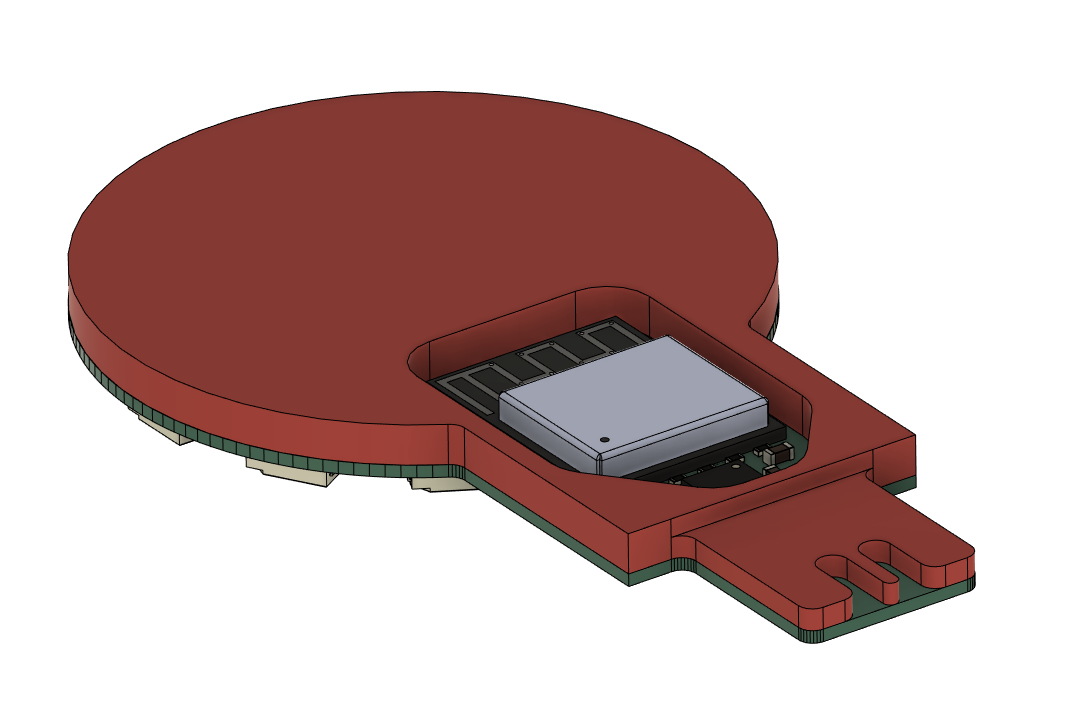
\includegraphics[width=0.6\textwidth]{text/PraktickaCast/img/SemiSemafor-vlozka.png}
  \label{semisemafor-vlozka}
  \caption{DPS Semisemaforu opatřena vložkou}
\end{figure}

\begin{figure}[!h]
  \centering
  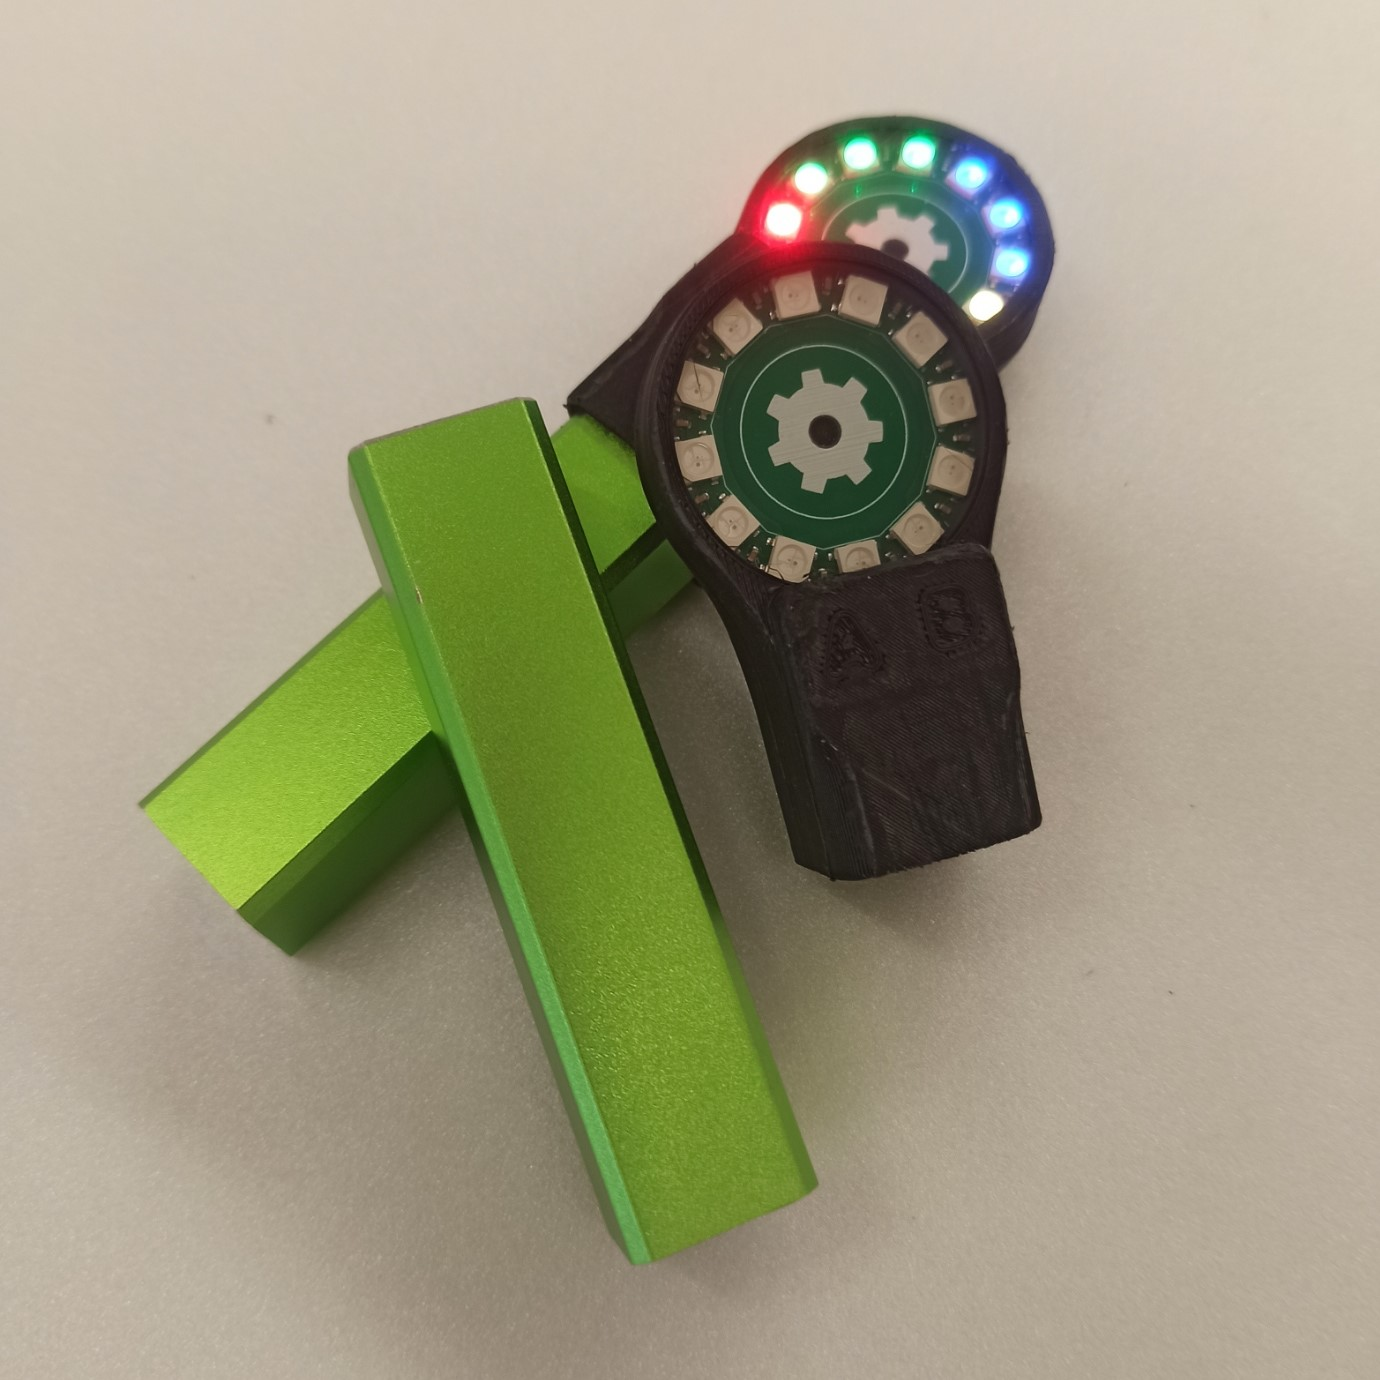
\includegraphics[width=0.8\textwidth]{text/PraktickaCast/img/Real-SemiSemafor.jpg}
  \label{semisemafor-real}
  \caption{Reální kus Semisemaforu}
\end{figure}

